\section{Frequentist Analysis}
\label{sec:frequentist}
\emph{In short: the likelihood maximized for the two charges together gives $N_s=15{,}328\pm133$ and $\hat A=-0.0441$ with Minos intervals; $A=0$ is rejected at $5.2\sigma$ and the interval has nominal coverage in $1000$ bootstrap replicas.}
The Frequentist analysis estimates \Araw by maximizing the extended unbinned likelihood of Eq.~\eqref{eq:likelihood} with \texttt{iminuit}~\cite{iminuit}; the uncertainty and the test of $A=0$ come from the profile likelihood, the other parameters being nuisance parameters (Secs.~\ref{sec:freq_model}--\ref{sec:freq_ci}).
\subsection{Mass Model and Fit Strategy}
\label{sec:freq_model}
\label{sec:freq_simfit}
The common mass model of Sec.~\ref{sec:model} (Eq.~\eqref{eq:mixture}) was fitted on $[5100,5600]\,\MeV$: a Gaussian signal with mean $\mu$ and width $\sigma$ shared by the two charges and a double-exponential background with shape and yield of its own for each charge, twelve parameters as in the Bayesian fit, through \texttt{iminuit.cost.ExtendedUnbinnedNLL}; the minimization started from an unbinned fit of the sidebands (the window without $[5200,5350]\,\MeV$). The asymmetry was estimated in two ways: in the \emph{simultaneous} fit the two charges share $N_s^\pm=N_s(1\mp A)/2$ and $A$ is a parameter of the likelihood; in the \emph{separate} fits each charge was fitted alone (seven free parameters each) and $\Araw=(N_s^--N_s^+)/(N_s^-+N_s^+)$ was computed from the two yields. They give $-0.0441\pm0.0085$ and $-0.0442\pm0.0087$: sharing $\mu$ and $\sigma$ between a particle and its antiparticle is adequate, and the simultaneous fit, which gives the profile-likelihood interval directly, is the \textbf{nominal} one. It gives $N_s=15{,}328\pm133$ and $N_b=4{,}403\pm82$, against the Bayesian posterior medians $15{,}328\pm133$ and $4404\pm82$ (Sec.~\ref{sec:bayes_posterior}). The shapes were not tuned on this fit, and the alternatives are systematic variants (Sec.~\ref{sec:syst}). The nominal fit has $\chi^2/\mathrm{ndof}=160/88$ ($p=4.8\cdot 10^{-6}$) in $2\times50$ bins of $10\,\MeV$; a single exponential is rejected ($294/92$, $p=5.7\cdot 10^{-23}$)\appref{sec:validation_gof} because the background rises towards the lower edge of the window (Sec.~\ref{sec:data_mass}). The fit of the two charges is shown in Fig.~\ref{fig:freq_jointfit}.

\begin{figure*}[t]
\centering
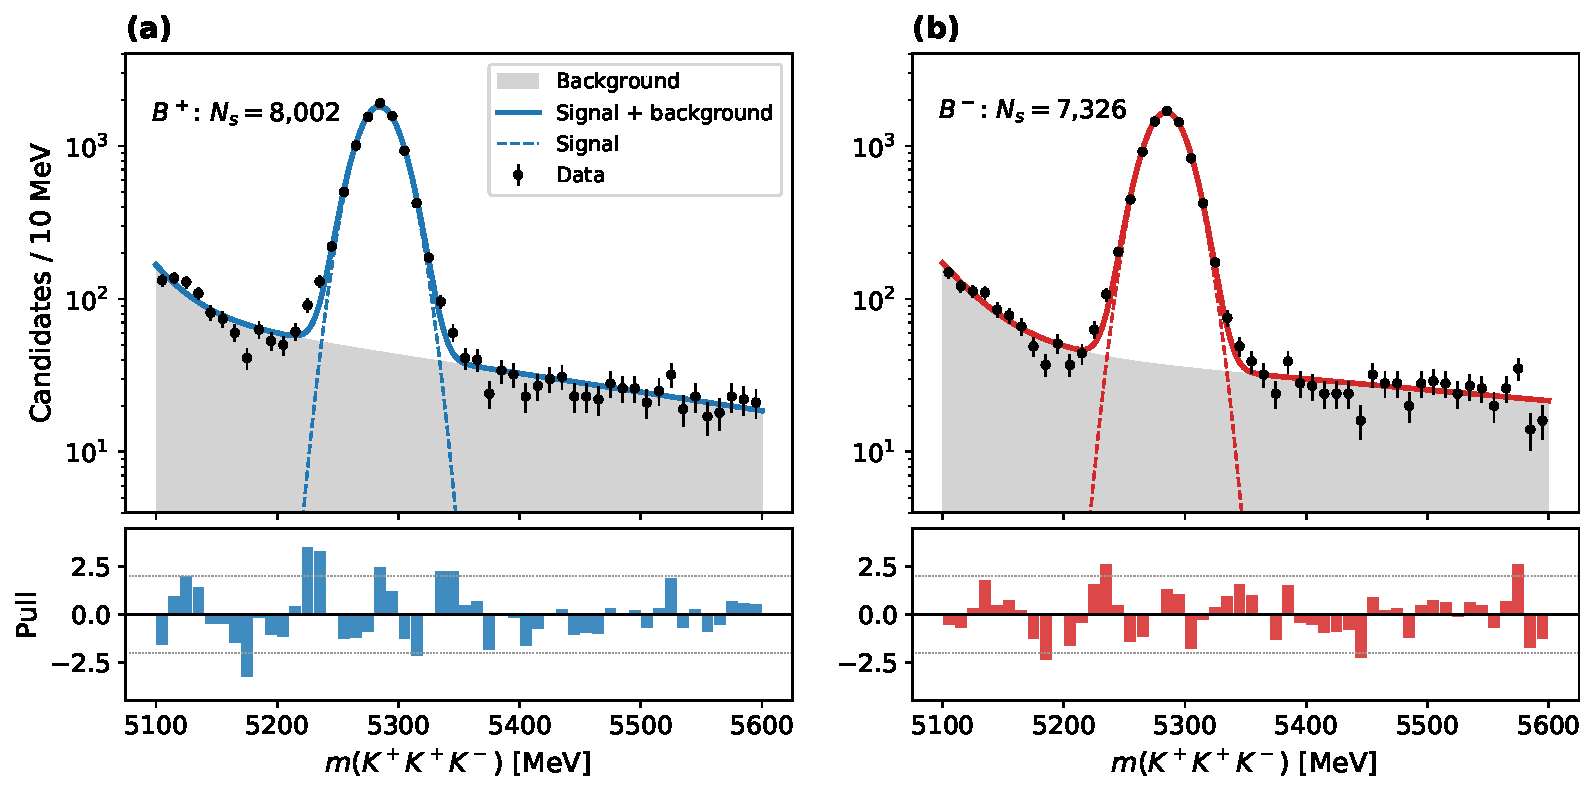
\includegraphics[width=0.95\textwidth]{figures/freq_jointfit.pdf}
\caption{Simultaneous fit of (a) $B^+$ and (b) $B^-$ in $10\,\MeV$ bins, logarithmic scale: data, signal (dashed), double-exponential background (grey) and their sum; below, the pulls $(n_i-\mu_i)/\sqrt{\mu_i}$ of the fit, with the $\pm2$ lines. The fitted signal yields are $8002$ and $7326$.}
\label{fig:freq_jointfit}
\end{figure*}

\subsection{Profile Likelihood and Confidence Interval}
\label{sec:freq_ci}
The maximum-likelihood estimate is \bnum{\hat A=-0.0441} (Hesse uncertainty $0.0085$), with \texttt{MINOS}~\cite{minuit} intervals $68\%$ CI $[-0.0526,-0.0356]$ and $95\%$ CI $[-0.0607,-0.0275]$; the uncertainties are statistical only (the systematic one is in Sec.~\ref{sec:syst}). The \emph{profile likelihood ratio} $q(A)=-2\log[L(A,\hat{\hat\theta})/L(\hat A,\hat\theta)]$, with the other eleven parameters re-minimized at each $A$ (\texttt{mnprofile}), is shown in Fig.~\ref{fig:freq_profile}; by Wilks' theorem~\cite{wilks} it follows a $\chi^2$ distribution with one degree of freedom at the true value of $A$, so the intervals are the sets $q\leq1$ and $q\leq3.84$. For the null hypothesis, $q(0)\simeq27$, $p=2.05\times10^{-7}$, \bnum{5.20\sigma}\appref{sec:appendix_freq}: no asymmetry is rejected, the counterpart of the Savage-Dickey test of Sec.~\ref{sec:bayes_factor} ($A=0$ at $5.2$ posterior standard deviations); the $p$-value is not the probability of $H_0$ and the Bayes factor depends on the prior width, but the conclusion is the same. The result agrees with the Bayesian one (Sec.~\ref{sec:bayes_posterior}: $-0.0443$, $68\%$ CI $[-0.0528,-0.0358]$), as expected with flat priors and $\sim2\times10^4$ events.

\begin{figure}[h]
\centering
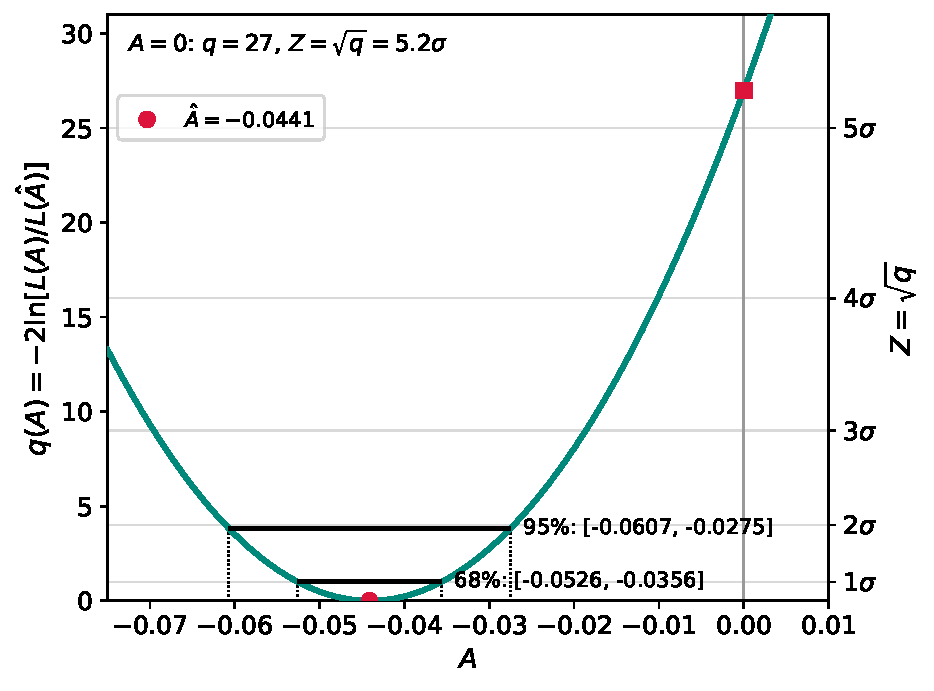
\includegraphics[width=\columnwidth]{figures/freq_profile.pdf}
\caption{Profile likelihood ratio $q(A)$ of the simultaneous fit, with the other eleven parameters re-minimized at each $A$ (right axis: $Z=\sqrt q$). The horizontal segments are the $68\%$ and $95\%$ Minos intervals ($q\leq1$, $q\leq3.84$); at $A=0$, $q\simeq27$, i.e. $5.2\sigma$.}
\label{fig:freq_profile}
\end{figure}

\subsection{Coverage of the Wilks Intervals}
\label{sec:freq_coverage}
Wilks' theorem is asymptotic, so the coverage was checked on the data with $1000$ bootstrap replicas of the $19{,}731$ candidates, refitting the nominal model on each (non-converged fits discarded); with $A_{\mathrm{true}}=-0.0441$, the $68\%$ interval of a replica contains it if and only if $q(A_{\mathrm{true}})\leq1$. The fraction is \bnum{68.4\pm1.5\%} against $68.3\%$ nominal (Fig.~\ref{fig:freq_toys}). It agrees with the toy-MC check of the Bayesian interval ($65.0\pm3.3\%$, $200$ experiments)\appref{sec:bayes_toymc}; the two checks are not equivalent, since the Bayesian pseudo-datasets come from the fitted model (a closure test) while the replicas are resampled from the data and carry the features that the model does not describe, such as the signal tails\appref{sec:bayes_gof}.

\begin{figure}[h]
\centering
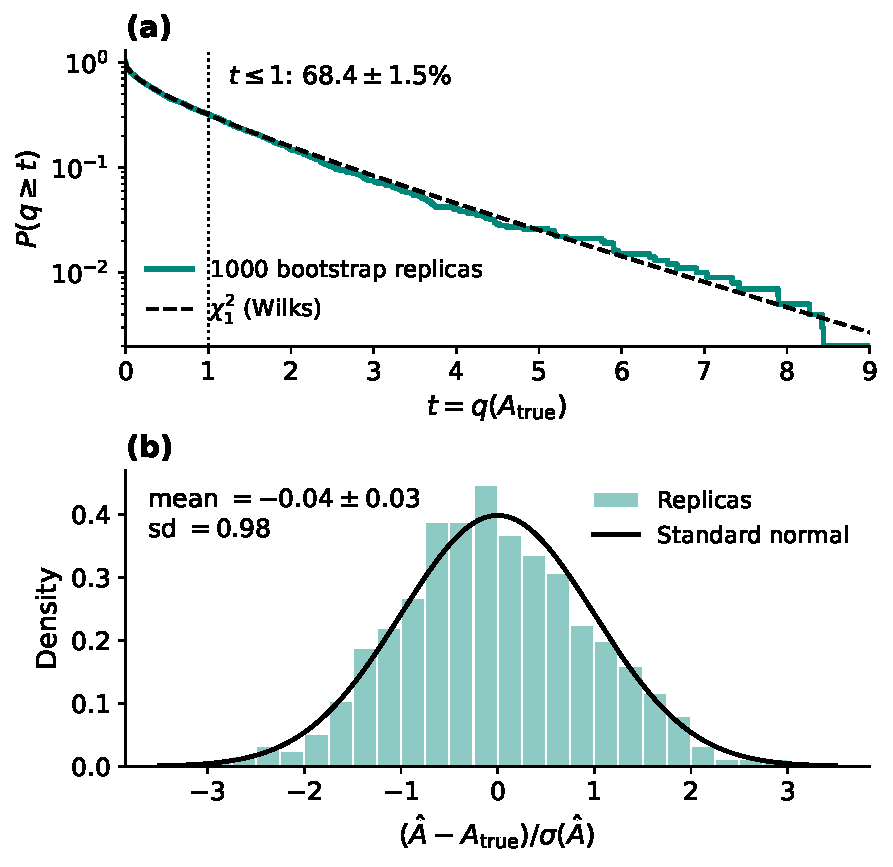
\includegraphics[width=\columnwidth]{figures/short_coverage.pdf}
\caption{Coverage check with $1000$ bootstrap replicas of the data. (a) Survival function of $t=q(A_{\mathrm{true}})$ against the $\chi^2_1$ distribution expected from Wilks' theorem; the dotted line is the $68.3\%$ limit ($t=1$). (b) Pulls $(\hat A-A_{\mathrm{true}})/\sigma(\hat A)$ of the replicas against a standard normal.}
\label{fig:freq_toys}
\end{figure}

\subsection{Additional Results}
\emph{Neyman construction and momentum.} Inverting the test of $A_{\mathrm{true}}$ with toy-MC experiments gives the same interval as the likelihood ratio, and $\Araw$ does not depend on the momentum of the $B$\appref{sec:checks_belt}.
\emph{Uncertainties of the twelve parameters.} The standard deviations from the Hesse matrix, the bootstrap of the data and the posterior agree for $A$, $A_b$, $\mu$ and $\sigma$; the bootstrap differs for the two yields, because it keeps the total number of candidates fixed, and for the weakly constrained steep slope $\lambda_1^+$\appref{sec:checks_covariance}.
\emph{Starting values.} $29$ of $30$ fits from random starting points reach the same minimum\appref{sec:checks_multistart}.
